\chapter{Search Engines} \label{chap:searchengines}

\begin{flushright}
    \textit{``A serious and good philosophical work could be written consisting entirely of jokes.''}
    \\ --- Ludwig Wittgenstein
\end{flushright}

%%%%%%%%%%%%%%%%% Information Retrieval
Information Retrieval (IR) is the data-driven field of Computer Science dedicated to creating systems that can retrieve specific piece(s) of information on request from within unfathomably massive bodies of information. It is integral to: genome mapping, spam filtering, plagiarism checking, recommendation systems (YouTube, Netflix, ...), and unsurprisingly: search engines, which are the primary focus of this thesis. Search engines are the IR systems that allow people to retrieve information from medical databases, academic libraries, and the World-Wide-Web. Commercial Search Engines include: PubMed, Google Scholar, and most notably Google Web Search\footnote{At the outset of my Master's research, I hoped Google would eventually hire me, but now I would rather keep my soul uncorrupted.}.

%%%%%%%%%%%%%%%%% Information Need
\section{Information Need}
When a user wishes to know something, we say they have an \textit{information need}; they desire to obtain some specific piece of information. A system created to satisfy an information need is called an Information Retrieval Engine or a Search Engine. What makes a good Search Engine? A quality search engine should be intuitive to use, quick to retrieve, also accurate and comprehensive in what it retrieves. For example, a doctor may have an urgent need to know the treatment for \textit{Chronic Decollatio}\footnote{What are the long term side-effects of decapitation?}. From a database of medical knowledge, a competent search engine would provide all possible treatment options. no more; no less. Retrieving \textit{all} the relevant information and \textit{only} the relevant information promptly and in a user-friendly way is a monumental task, considering the potentially tremendous amount of data to be sifted through.
%Factor (1) is preferential, (2) is relativistic, (3) and (4) however are crucial, and are usually called \textit{recall} and \textit{precision}.

For Web Search, a user's intent is commonly classified into these three broad categories: Informational, Transactional, and Navigational \cite{broder2002taxonomy}. Navigational intent is when a user does not know, forgot, or cannot be bothered typing a web URL. Transactional intent indicates the user is looking for a web service or resource, e.g. ecommerce purchase. Finally, Informational intent is when a user wishes to learn something. In web search, around 50\% \cite{broder2002taxonomy} and 80\% \cite{jansen2008determining} of all web searches have informational intent; they are also the hardest to monetise\footnote{But not impossible, e.g.\ obscuring academic papers behind a paywall.}.

% This thesis will disregard both transactional and navigational as data-sets for these tasks are kept secret by commercial entities.

%%%%%%%%%%%%%%%%% Search Queries
\section{Search Query}
Before the search engine can fulfil any informational requirements, the user must communicate their desire(s) through a request known as a \textit{search query}. The query is a representation of their information need, which is understandable by the search engine. Queries are often expected to be plain text but could be any form of media (e.g.\ image, sound clip). Text queries can be processed by one of three main retrieval systems: knowledge, data, and text \cite{lewis1996natural}.

%%%%%%%%%%%%%% KNOWLEDGE RETRIEVAL
\textbf{Knowledge retrieval} is the most sophisticated of the three and requires complex linguistic comprehension of the query. From answering simple trivia questions to more abstract problem solving, knowledge retrieval aims to emulate the cognition of a human mind if it were infallible and more omniscient. Deep learning's advances in Natural Language Understanding (NLU) approaches (e.g.\ OpenAI's GPT or BERT) already outperform non-experts \cite{wang2019superglue}. After the query has been \textit{``understood''}, the system then traverses a highly structured and content-rich ontology (knowledge graph) to \textit{generate} an answer specific to the user's request. Commercial examples include Google's Knowledge Graph \cite{singhal2012introducing}, and WolframAlpha, the freely available Computational Knowledge Engine \cite{wolfram2012wolframalpha}.

% \footnote{These systems struggle at identifying nonsense, for example, I asked WolframAlpha ``how many years between 11 April 1994 and the height of Mount Everest?'', and it replied ``16.75 years"}

%%%%%%%%%%%%%% DATA RETRIEVAL
\textbf{Data retrieval} also makes use of structured information: spreadsheets, relational databases, or even ontologies. The main distinction from knowledge retrieval is that the queries require a structure that is not a natural language, e.g. Structured Query Language (SQL) for Relational Databases. These formal query languages are technical in nature and are not intuitive to use. Not only must the query language's grammar be learned, but specifics of the data structure must also be known. Therefore, the barrier to entry for the average user is reasonably high. Another difference is that the system does not generate information per se; it can only retrieve a subset of its containing data. The caveat is some fancier query languages allow for explicit processing directives, which perform minimal computations on the retrieved data.

% . An ideal search engine would be able to understand unstructured and arbitrary queries, i.e.\ written in a human language.

%%%%%%%%%%%%%% TEXT RETRIEVAL
\textbf{Text retrieval} is the most common system. It is designed for unstructured, semi-structured, or information that has a structure but is unknown to the retrieval system. This makes it ideal for websites, newspapers, books, and any other text document format. This is why it is often called \textit{Document retrieval}. Although text retrieval usually retrieves entire documents, there is also \textit{Passage Retrieval} which retrieves excerpts from within documents. Text retrieval performs search tasks not through \textit{``understanding''} information but rather through probabilistic assumptions between the user's query and the relevant documents.

\begin{table}
\begin{center}
\begin{tabular}{l|l|l|}
\cline{2-3}
                                          & Query                     & Information                    \\ \hline
\multicolumn{1}{|l|}{Knowledge Retrieval} & Natural Language          & Complex data structure         \\ \hline
\multicolumn{1}{|l|}{Data Retrieval}      & Structured                & Simple data structure          \\ \hline
\multicolumn{1}{|l|}{Text Retrieval}      & Unstructured (ad-hoc)     & Unstructured / Semi-structured \\ \hline
\end{tabular}
\end{center}
\caption{Comparison of retrieval types} \label{tab:retrievaltypes}

\end{table}

Many text retrieval systems support meta directives, much like data retrieval. For example, \textit{Boolean Retrieval} supports boolean operators within the query, e.g.\ the NOT operation excludes query terms. Most commercial systems support various directives to help the IR system, including ``double quotes'' that make terms required and/or define their order.

%%%%%%%%%%%%%% ADHOC QUERIES
The queries in text retrieval are unstructured, much like knowledge retrieval. The query is required only to be a string of word(s); however, there is no expectation the user will adhere to the language's grammar rules or even be comprehensible by conventional standards. This is often called \textit{ad-hoc retrieval}, and a series of keywords is often sufficient to form an ad-hoc search query. Most contemporary internet search engines accept this kind of free-form query construction. A query has a much higher chance of success if it is somewhat well-formed, but a quality search engine can handle typos, misspellings, even incomprehensible gibberish. For example, if one types a query into Netflix by mashing the keyboard in the chaotic, higgledy-piggledy manner of a fat-fingered, drunken animal:

\begin{center}
    % ``''a3857vb349se7itn7o834tcyweufhsldjkghancrauawmefhsceukt''
    ``asdf;ksa;llfsdfsadfasdk;lfjasjfdk;lasfjldfjsafjdsl;fjajfdlksaj''
\end{center}

\noindent
Netflix will suggest children’s TV shows.

% , which is a feature to be applauded. 

% Netflix will also auto complete titles for movies it doesn't have, which is annoying.

\subsection{Unstructured Information}
Internet websites are the most accessible source of unstructured information, but they are not the only type. An information retrieval system can be constructed for any digital information store, so long as the information store can be discretized into a collection of documents. The content of a single document varies depending on the information domain (e.g.\ academic journals, web pages, images, audio files). Herein we will be focusing only on text documents for text retrieval. The grammar in text documents is ignored by default; they are considered a mere sequence of words (\textit{lexical tokens} or \textit{terms}). Documents may also be considered semi-structured, which is when parts of documents (e.g.\ headings, sections, paragraphs) have been tagged (e.g. XML).

The collection of all documents accessible to the IR system is called the \textit{corpus} or \textit{document collection} and is often massive, in the order of multiple gigabytes in size and potentially significantly larger. We will not be discussing the processes involved in acquiring a collection or adding structure to the documents. You may: scan books at your local library, illegally download ebooks from \textit{Library Genesis}\footnote{Libarary Genesis is located at libgen.is should you wish to avoid it.}, or flout the temporal boundaries of reality to recover scrolls from The Great Library of Alexandria\footnote{I am seeking a research grant for this project.}. We only require that the documents be converted into digital files so that they can be searched.

%%%%%%%%%%%%%% TERM MATCHING
\section{Estimating Relevance}
Documents are considered relevant if they satisfy a user's information need. It is a binary value judged by the user themselves, either explicitly stated in user studies or implicitly assumed from the user's behaviour. A text retrieval system cannot ever know for certain which documents are relevant, there is always an amount of uncertainty. The output of a relevance model\textemdash Retrieval Status Value (RSV)\textemdash is interpreted as an indicator of relevance, or the probability of relevance, as outlined in the Probability Ranking Principle \cite{jones2000probabilistic} (PRP). There are many relevance models which all essentially perform the same task, they compute some statistical similarity between the document vocabulary and the query vocabulary. For example, if the document contains most (or all) of the query's terms, then the document is assumed to be relevant to the information need. 

% You may have already started to doubt the effectiveness of inferring relevance via a vocabulary comparison, however PRP is proven very effective in practice and the blame for any retrieval failure is placed squarely on the users who construct inadequate search queries (we will explore this topic later).

% Term Matching, Vector Space, Language Modelling

% \textbf{Document Clustering}

\subsection{Term Matching Model}
Term matching estimates relevance by directly matching document terms with query terms, i.e.\ the terms that co-occur in both the document and the query. The document which contains the most query terms is considered the most relevant. The document which contains the fewest or no query terms is considered the least relevant. In short relevance of a document is proportional to the frequency of query terms. Query terms are connected with an implicit OR, so it is not required that every query term occurs in the document. 

% Also known as \textit{Boolean model} or \textit{keyword matching}.

Na{\"i}vely searching through each document in the collection and counting the occurrence (frequency) of each query term can be too slow for interactive search, which is why term matching implementations precompute an index from the collection. The index structure most commonly used is the Inverted File which is much like the index at the back of a book, except instead of a minimal set of keywords, every word in the collection vocabulary gets an entry in the alphabetised list. Each entry in the Inverted File has an associated \textit{posting list} which lists every document that the term appears in, along with the term frequency ($\mathit{tf}$). Our example documents will be ``fruits.txt'', ``iPod.doc'', and ``apple-pie.pdf'' with respective document ids: 1, 2, and 3. If the word ``apple'' appears five times in the document ``fruits.txt'', 12 times in the document ``iPod.doc'', and eight times in the document ``apple-pie.pdf'', then the posting list for the entry ``apple'' might look like this:

\begin{center}
    index\big[ ``apple'' \big] $\Rightarrow$ \big[ (1, 5), (2, 12), (3, 8) \big]
\end{center}

Now, if a query includes the term ``apple'', the system need only find the entry for ``apple'', which is quick given that the entries are alphabetised, then provide the user with the three document ids in the postings list. An index may also record the document frequency ($\mathit{df}$), which is the number of documents that contain a particular term. For ``apple'' the $\mathit{df}$ would be 3.

\subsection{Vector Space Model} 
An alternative to term matching as a relevance model is Vector Space. Imagine a multidimensional space, V-dim, where every unique word in the collection vocabulary has its own dimension. Documents and queries can be placed in this space where their coordinates on each axis are equal to the frequency of each word in the document. Relevance is estimated from cosine similarity within the vector space or the Euclidean distance if we normalize for document length. 

% Another vector space approach uses machine learning to find vector representation of words e.g.\ Google's Word2Vec and Facebook's fastText.

% Something about clustering?

% Something about Binary Independence Model

\subsection{Query Likelihood Model}
The third relevance we will look at is based on Language Modeling (LM). The Query Likelihood Model considers sequences of words as conditional probabilities. Language Models have seen huge success in speech recognition, search engine autocomplete, and predictive text on smartphones. 

Let us consider a language model not as a word predictor but rather as a random word generator, and every unique document in our collection has been generated by a unique LM. Each of these LMs can be prompted to generate a string of words that have the same vocabulary distribution as the original document\footnote{I attempted to generate jokes with a Markov chain implementation of an LM with zero success.}. Each word does not have an equal chance of being generated, but rather each word's probability is relative to its occurrence in the original document. For example, the language model for The Holy Bible would generate the word \textit{``miracle''} more frequently than the language model for Darwin's On the Origin of Species (specifically 4x higher, see Table \ref{tab:miracle}). A language model for Islamic religious texts would likely generate the phrase \textit{``Peace be upon him''} immediately after generating the word \textit{``Muhammad''}, as it is the Durood Shareef tradition prolific in Islam. 

The Query Likelihood Model estimates a document's relevance by the likelihood that its language model would generate the user's search query. Most language modelling implementations for IR are unigram models or \textit{Bag-of-words} models, which assumes the word order and grammar are not important, but the occurrence (or frequency) of each word is important. Unigram models are often sufficient for text retrieval as queries are considered to be ad-hoc. Bi-gram and n-gram models account for word order, but they are much less efficient and suffer from data sparseness, i.e.\ documents and collections too small to calculate comprehensive and accurate models from.

\begin{table}
    \begin{center}
        \begin{tabular}{llll}
        \cline{2-4}
            \multicolumn{1}{l|}{}
            & \multicolumn{1}{l|}{The Holy Bible}
            & \multicolumn{1}{l|}{Origin of Species}
            & \multicolumn{1}{l|}{This Document}
        \\ \hline
            \multicolumn{1}{|l|}{Word count}
            & \multicolumn{1}{l|}{727,969}
            & \multicolumn{1}{l|}{208,415}
            & \multicolumn{1}{l|}{32,382}
        \\ \hline
            \multicolumn{1}{|l|}{\textit{``miracle''} count}
            & \multicolumn{1}{l|}{42}
            & \multicolumn{1}{l|}{3}
            & \multicolumn{1}{l|}{17}
        \\ \hline
            \multicolumn{1}{|l|}{\textit{``the''} count}
            & \multicolumn{1}{l|}{83,702}
            & \multicolumn{1}{l|}{14,581}
            & \multicolumn{1}{l|}{1,782}
        \\ \hline
            \multicolumn{1}{|l|}{\begin{tabular}[c]{@{}l@{}}\textit{``miracle''} proportion\end{tabular}}
            & \multicolumn{1}{l|}{0.0000576}
            & \multicolumn{1}{l|}{0.0000144}
            & \multicolumn{1}{l|}{0.0005475}
        \\ \hline
            \multicolumn{1}{|l|}{\begin{tabular}[c]{@{}l@{}}\textit{``the''} proportion\end{tabular}}
            & \multicolumn{1}{l|}{0.1150}
            & \multicolumn{1}{l|}{0.0699}
            & \multicolumn{1}{l|}{0.0550}
        \\ \hline
        \end{tabular}
    \end{center}
\caption{Word counts of ``miracle'' and ``the'' in \textit{The Holy Bible} (NIV edition), \textit{On the Origin of Species} (6th Edition), and this document itself.} \label{tab:miracle}
\end{table}

\section{Ranking}
The core of any Search Engine is the ranking function. It is the algorithm that calculates the relevance score for each document, then sorts the documents by descending relevance. The document with the highest relevance score is placed in the top rank; the second most relevant document gets the second rank, etc... A fast and simple ranking function is sorting by term frequency, i.e. the document which contains the most query terms is ranked the highest. However, this simple approach is not the most accurate. Currently, the most accurate way to rank documents is with machine-learned ranking (MLR) or learning to rank methods. The downside to MLR is the comparatively slow speed on massive document collections. For interactive web search, users expect retrieval results in a few milliseconds, and the web contains billions of documents, which is why modern web search performs ranking using both MLR and more simple ranking algorithms \cite{baeza1999modern}. This is known in the literature as a multi-tier ranking pipeline \cite{risvik2003multi}, a cascade of document filters incrementally reduce the document collection into a more manageable size. The lowest tier performs top-$k$ document retrieval, reducing billions of documents down to a few million (or a few thousand). This smaller subset of the document collection is then re-ranked in the higher tiers with much slower but far more accurate MLR methods. The focus of this thesis is on the lowest tier of the ranking pipeline.

% then a final optional phase involves manipulating the top results depending on how much each document author has \st{bribed} paid the search engine provider.

% Web Search is usually performed on distributed architecture due to the vast nature of the collection
% Fagin's algorithm, Threshold Algorithm (TA), probabilistic TA sorted, Linear Programming adaptation of TA

% Google Web Search uses the proprietary PageRank algorithm, technically nobody outside of Google knows how it works... but in theory, web pages are ranked higher relative to how much you bribe the grubby, money-hungry fuck pigs who run Google.

% One could rank based on the output of your chosen relevance model alone (Vector, Likelihood, or term matching)


\subsection{TF-IDF Ranking}
Na{\"i}ve ranking assumes that all words in a language are of equal importance, which they are not, as some terms are more \textit{discriminating} than others. The most common word in both Darwin's seminal book and The Holy Bible is \textit{``the''}, occurring roughly once every 10-16 words (see Table \ref{tab:miracle}). This probability is similar for many documents written in English. If a query and a document contain the term \textit{``the''}, it does not necessarily indicate relevance to the information need as most documents contain the word \textit{``the''}. We are most interested in terms that uniquely identify, what we might call \textit{discriminating terms} or \textit{content bearing terms}. These words are identified by being uncommon across the collection but overly-prevalent in specific documents. A word like \textit{``miracle''} fits the description and would easily discriminate documents about miracles from documents with no association with miracles\footnote{According to Table \ref{tab:miracle}, the word \textit{``miracle''} is more prevalent in this document than The Bible. Is this document about miracles? The fact I managed to finish this thesis is rather miraculous.}.

The most common words in a document collection are called \textit{stop words}. They may be explicitly excluded in a relevance model as they are almost always grammar particles (e.g.\ articles, conjunctions, prepositions) and carry little to no information. However, US linguist George Zipf has provided a much better way to handle these common words in what is known as Zipf's law \cite{zipf1949human}, which is analogous to findings by Claude Shannon described independently around the same time \cite{shannon1948mathematical}. It is a language phenomenon that is proven to be found in over 50 human languages \cite{yu2018zipf}. Zipf's law was brought in to IR research in 1972 by Karen Sp{\"a}rck Jones \cite{jones1972statistical}, who stated that if we plot the rank of words in decreasing order against their frequency, it matches a discretized power law. There is an exponential relationship between a word's occurrence across a document collection and its ability to discriminate documents.

Sp{\"a}rck Jones suggested that terms could be weighted by the inverse of their collection frequency, as a measure of term specificity, which later became known as \textit{inverse document frequency} or IDF. It is normally calculated as the total number of documents $N$ divided by the number of documents which contain the term ${df_{t}}$. If terms are weighted by their IDF, it will boost the contribution of content bearing terms and diminish the contribution of non-discriminating terms, which has proved to be extraordinarily robust and forms the basis of the many ranking functions in use today: TF*IDF, which sums the product of each query term's frequency ($\mathit{tf}_{td}$) with the IDF.

\begin{equation} \label{tfidf}
    rel(d) = \sum_{t \in Q} \mathit{tf}_{td} \times \frac{N}{df_{t}}
\end{equation}

Improvements on Sp{\"a}rk's IDF include taking the log of the quotient, as the contribution of inverse document scores do not scale linearly but rather sub-linearly. Also, the inclusion of parameters for the estimated number of relevant documents and smoothing corrections \cite{robertson1976relevance, robertson1997relevance}, known in the literature as the Robertson-Sp{\"a}rck Jones (RSJ) weight.

\begin{equation} \label{tfidfrsj}
    rel(d) = \sum_{t \in Q} \mathit{tf}_{td} \times \log_{10}\left(\frac{N - df_{t} + 0.5}{df_{t} + 0.5} + 1\right)
\end{equation}

This allows content bearing terms to have a larger contribution to the relevance estimate, and common words like \textit{``a'', ``the''}, and \textit{``and''} to have negligible contribution.

% The IDF component scales the RSV by taking into account the frequency of a query term across the entire document collection. If a term is contained within the majority of the collection (e.g.\ `the'), it is not considered a discriminating term, so its contribution to the RSV is negligible. But if the term is only contained within few documents, then it is considered highly discriminating, and has a large contribution to the final RSV. 

% hapax legomena
% Google Whack














\subsection{Okapi BM25}
TF*IDF has many variants and influences, including Okapi BM25, one of the most successful retrieval models. Okapi BM25 (BM25) is a probabilistic relevance ranking algorithm devised by Robertson and Walker in 1994 \cite{robertson1995okapi}. Its mathematical foundation is a unigram Language Model based on research by Harter \cite{harter1975probabilistic}, who showed that a document's terms could be modelled as a mixture of two distributions, each with different means. One distribution of terms appears uniformly random across the document collection and provides little value for search, and the other distribution of \textit{specialty} terms which are far more valuable for search. BM25 assumes that all term frequencies conform to a Poisson distribution, a discrete probability distribution where subsequent document terms are modelled as events in time.

%%%%%%%%%%%%%%%%%%%%%% Aboutness
The other key idea of BM25 is the notion of \textit{eliteness}. Every term in the collection vocabulary is thought to represent a concept. Each document can be \textit{about} one or more concepts, where \textit{aboutness} is an unknown feature of documents. If a term appears in a document and the document is \textit{about} the term's concept, then the term is \textit{elite} for that document. For example, both The Holy Bible and Darwin's Origin of Species contain the term \textit{``miracle''}. However, only The Holy Bible is \textit{about} miracles. Darwin's book is not \textit{about} miracles. So the term \textit{``miracle''} is elite in The Holy Bible, and it is not elite in Darwin's book\footnote{This example was chosen intuitively as an illustrative example but is also mathematically sound.}.

BM25 treats documents as a linear combination of two Poisson distributions, one distribution for elite terms, the other distribution for non-elite terms; see Figure \ref{bm25poisson}. Since \textit{aboutness} is unknown to the retrieval system, the eliteness is a hidden variable. It is also a binary variable; either a document is \textit{about} a concept or not, the term belongs to either one of the Poisson distributions. Relevance is estimated from the probability of term eliteness rather than term frequency directly \cite{bookstein1974probabilistic, harter1975probabilistic, robertson1995okapi}.

% 0.0028, k1 = 6.4691
\pgfmathdeclarefunction{poiss}{1}{%
  \pgfmathparse{(#1^x)*exp(-#1)/(x!)}%
  }
\begin{figure}
  \caption{BM25's 2-Poisson term distribution(s)} \label{bm25poisson}
  \begin{tikzpicture}
        \begin{axis}[
            height=5cm,
            width=\columnwidth,
            % axis x line=center,
            axis y line=center,
            axis x line=left,
            xtick={0,2,...,19},
            ytick={0.2, 0.4, 0.6, 0.8},
            domain = 0:10,
            samples = 11,
            xlabel style={align=center},
            % xlabel style={text width=8cm},
            xlabel={$\mathit{tf}_{\!\!td}$ : Frequency of term $t$ in document $d$.},
            % xlabel style={right},
            yticklabel style={
                /pgf/number format/fixed,
                /pgf/number format/precision=3,
                /pgf/number format/fixed zerofill
            },
            scaled y ticks=false,
            ylabel style={above}, %rotate=-90},
            ylabel={$P(\mathit{tf}_d|E)$},
            ymax=1, %0.005,
            xmax=10,
            % x post scale=1.4,
            legend cell align={left}
            ]
            \addplot+[blue, mark=*] {poiss(0.25) + poiss(2.5)};
            % \addplot[blue] {poiss(0.25) + poiss(2.5)};
            \addlegendentry{2-Poisson};
            \addplot+[red, mark=square*] {poiss(0.25)};
            % \addplot[red] {poiss(0.25)};
            \addlegendentry{non-elite terms ($E=0$) }
            \addplot+[violet, mark=triangle*, mark options=solid] {poiss(2.5)};
            % \addplot[green] {poiss(2.5)};
            \addlegendentry{elite terms ($E=1$)};

        \end{axis}
    \end{tikzpicture}
\end{figure}

% • Relevance to a query is related to eliteness rather than directly to term frequency, which is assumed to depend only on eliteness.

% term frequencies depend only on eliteness

% • Hypothesize that occurrences of a term in a document have a random or stochastic element

%%%%%%%%%%%%%%%%%%%%%% Features of BM25

\begin{equation} \label{eq:BM25}
	RSV(d) = \sum_{t \in Q}
	\text{IDF}(t) \times
	\frac{(k_1 + 1) \times \mathit{tf}_{\!\!td}}{k_1 \times \Big((1-b) + b \times \Big(\frac{L_d}{L_{avg}}\Big) \Big) + \mathit{tf}_{\!\!td}} 
\end{equation}

In practice, BM25 can be viewed as an extended TF-IDF model, see Equation~\ref{eq:BM25}. It performs a sum over every term $t$ in the query $Q$, where each summand is a product of an Inverse Documents Frequency (IDF) component and a Term Frequency (TF) component. 
% The original TF-IDF model was based on intuition and experimental research as was BM25, however BM25 has since a strong theoretical foundation \cite{idftheory}.
The IDF component is usually a variant of the RSJ weight, and the TF component is the 2-Poisson representation of the LM. BM25 provides two tunable parameters. The first is $k_1$, which controls the \textit{saturation point}. Saturation is a feature that asymptotically diminishes the contribution of large term frequencies as probabilistic relevance does not scale linearly with an increase in $\mathit{tf}$, but rather sub-linearly. For example, the manual for my car mentions the term \textit{``Tesla''} orders of magnitude more frequently than most online reviews about my car. However, the manual is not orders of magnitude more relevant to the query: \textit{``Tesla model S 100D review''}. The main benefit of the asymptotic limit is to prevent over boosting. If this is not done, we risk one of the query terms dominating the rank and the less frequent \textemdash but equally important\textemdash terms having a relatively inconsequential contribution. 

The shape of the saturation function can be clearly visualized by fixing the parameters and plotting RSV against $\mathit{tf}$, which can be seen in Figure~\ref{tfm}. It is clear that the first few occurrences of term $t$ have the largest effect, after $\mathit{tf}_{\!\!td} > 10$ the RSV begins to plateau. Figure~\ref{tfm} also compares the BM25 to unmodified TF*IDF, which increases without bound.

%$L_d = L_{avg}$, $k_1 = 0.9$, $b = 0.4$, asymptote at $k_1+1$.
% Parameters fixed for simplicity: $L_d = L_{avg}$, $k_1 = 0.9$, $b = 0.4$.

\begin{figure}[h]
% \baselineskip
% \baselineskip
% \vspace{-1cm}
  
  
  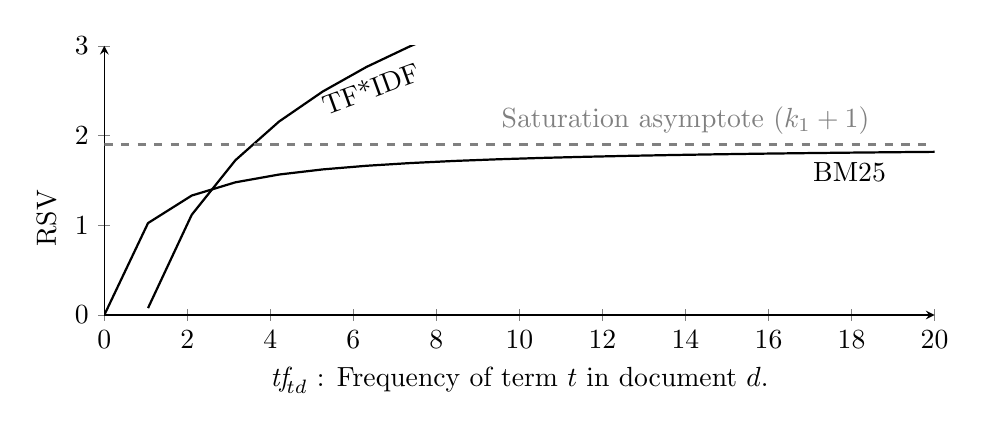
\begin{tikzpicture}
    \begin{axis}[
    	height=5cm,
        width=\columnwidth,
        xmin=0, xmax=20,
        ymin=0, ymax=3,
        % axis x line=center,
        % axis y line=center,
        axis lines = left,
        xlabel style={align=center},
        ylabel style={above left},
        % xlabel style={text width=8cm},
        xlabel={$\mathit{tf}_{\!\!td}$ : Frequency of term $t$ in document $d$.}, 
        ylabel={RSV},
        % title={\Large{BM25 term frequency component}},
        samples=20]
        \addplot[black, thick, domain=0:20, range=0:3] {ln(x) * 1.5} node[below,pos=0.3, rotate=20] {TF*IDF};
        \addplot[gray, thick, dashed, domain=0:20, range=0:2] {1.9} node[above,pos=0.7] {Saturation asymptote ($k_1 + 1$)};
        \addplot[black, thick, domain=0:20, range=0:2] {(x*1.9)/(x+0.9)} node[below,pos=0.9] {BM25};
        
      
    \end{axis}
  \end{tikzpicture}
  \caption{Comparing TF*IDF with BM25 ($L_d = L_{avg}$, $k_1 = 0.9$, $b = 0.4$)} \label{tfm}
\end{figure}


%%%%%%%%%%%%%%%%%%%%%% Document Length

The other parameter $b$, controls document length normalization. Early IR research was intended for small documents, e.g. titles and abstracts, but with the scale of the internet and faster computers, it has become expected to search on book-length documents. BM25 is indifferent toward document length ($L_d$) since it normalizes for average document length ($L_{avg}$). The parameter $b$ adjusts the influence of the normalization for collection-specific tuning ($b=0.75$ by default). 

The effect of different document lengths can be seen in Figure \ref{bm25doclen}. The document that is four times the average length takes many more terms to reach saturation, and the shorter document requires fewer terms to reach saturation. This makes intuitive sense since shorter documents contain fewer terms, it should not require as many terms to be confident the document is relevant. Much longer documents like books necessitate a much larger $\mathit{tf}$ to be confident in the relevance. The longer a document is, the more likely it will contain infrequent uses of words that falsely appear to be content-bearing terms but used in non-elite ways, possibly in metaphorical ways, e.g. \textit{``miracles of nature''}.

\begin{figure}
% \baselineskip
% \baselineskip
% \vspace{-1cm}

  
  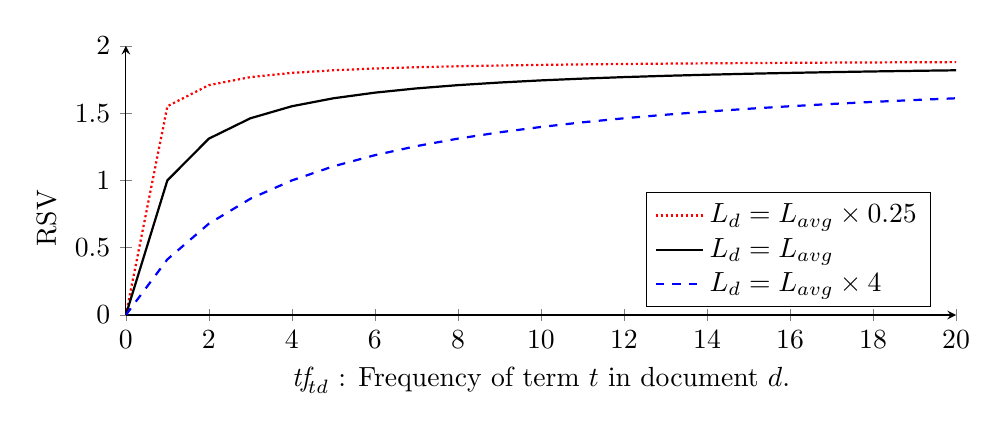
\begin{tikzpicture}
    \begin{axis}[
    	height=5cm,
        width=\columnwidth,
        xmin=0, xmax=20,
        ymin=0, ymax=2,
        % axis x line=center,
        % axis y line=center,
        axis lines = left,
        xlabel style={align=center},
        ylabel style={above left},
        % xlabel style={text width=8cm},
        xlabel={$\mathit{tf}_{\!\!td}$ : Frequency of term $t$ in document $d$.}, 
        ylabel={RSV},
        % title={\Large{BM25 term frequency component}},
        samples=21,
        legend pos=south east,
        legend cell align={left}
        ]
      \addplot[red, thick, densely dotted, domain=0:20, range=0:2] {(x*1.9)/(x + 0.9*(0 + 1*0.25))};
      \addlegendentry{$L_{d} = L_{avg} \times 0.25$}
      \addplot[black, thick, domain=0:20, range=0:2] {(x*1.9)/(x + 0.9*(0 + 1*1))};
      \addlegendentry{$L_{d} = L_{avg}$}
      \addplot[blue, thick, dashed, domain=0:20, range=0:2] {(x*1.9)/(x + 0.9*(0 + 1*4))};
      \addlegendentry{$L_{d} = L_{avg} \times 4$}
    \end{axis}
  \end{tikzpicture}
    \caption{Varying document length ($L_d$) in BM25 ($k_1=0.9$, $b=1.0$) } \label{bm25doclen}
\end{figure}

% Other ranking function may also consider the position of the query terms within the document, in which case the posting lists of the index must record the position(s) of the terms alongside the term frequency.

% Retrieval Status Value (RSV)



% \begin{equation} \label{BM25}
% 	RSV(d) = \sum_{t \in Q}
% 	\log_{10}\left(\frac{N - df_{t} + 0.5}{df_{t} + 0.5} + 1\right)
% 	\times
% 	\frac{
% 	    (k_1 + 1) \times \mathit{tf}_{\!\!td}
% 	}{
% 	    k_1 \times \Big((1-b)+b \times \Big(\frac{L_d}{L_{avg}}\Big) \Big) + \mathit{tf}_{\!\!td}
% 	}
% \end{equation}
% 	\times
% 	\frac{(k_3 + 1) \times qtf_t}{k_3 + qtf_t}

% Original Okapi: k1 = 2, b=0.75

% BM25: k1 = 1.2, b=0.75

BM25 has many features which make it ideal for practical implementations and not just theoretical musings. If $\mathit{tf} = 0$ then the retrieval score will also be zero. The RSV increases monotonically with term frequency, i.e.\ a rise in $\mathit{tf}$ will never reduce the retrieval score. Both vector space and language modelling have influenced BM25 and its extensions. 


\section{Problems With Relevance Models}\label{problems-with-relevance-models}
%%%%%%%%%%%%%%%%%%%%%%% short queries
One issue with ad-hoc retrieval is that it expects users to write adequate search queries. Unsurprisingly users often fall short of expectations. Firstly, their queries are very short. The majority of all queries contain only one, two, or three terms \cite{gabrilovich2009classifying}. According to Rand Fishkin, 79.18\% of Google's web search queries contain three or fewer terms, and searches performed from mobile phones have even fewer terms on average \cite{enge2012art}. With fewer search terms, the probability of them co-occurring within documents is clearly lower than would be expected of a more comprehensive search query.

But the wider problem is using vocabulary to estimate relevance as it makes two assumptions. The first is that the information content of a document is adequately described by the vocabulary it contains. The second is that the information need of a user is adequately described by the vocabulary the query contains. Individually, these assumptions appear to be entirely reasonable, especially when considering a human reader comprehending the information content. However, there is an unfortunate disparity that arises when both of these assumptions are made. Essentially, the query is written by someone ignorant about the vocabulary used in the document collection. And conversely, the document authors cannot predict what vocabulary might appear in a search query.

An extreme example of this disparity is obvious when considering the foreign language barrier. If a monolingual English speaker searches for marital guidance, they can type no query that will ever retrieve something written in Arabic, no matter how relevant the Arabic document may be. This is a shame, as the Qur'an has many great passages on marriage. That is not a glib joke. The Qur'an's reformation of marriage was progressive for its time: it forbade incestuous marriage (Qur'an 4:23); forbade forced marriage (Qur'an 2:232); though it also allows men to have up to four wives (Qur'an 4:3), no reasonable person would expect a 1,400-year-old moral codebook to perfectly espouse modern ideals. At least it does not promote forced incest, like Christian Royalty in England practised.

%%%%%%%%%%%%% MISCOMMUNICATION.... leads to vocabulary emismatch
%%% different authors, disparity, 

%The user is by definition ignorant, they lack some knowledge, specifically the piece of information they are seeking. The user hopes that there exists (or has existed) a person who is not ignorant and has at some point in the past written the piece of information they need within some document in thecollection. There is no guarantee that thecollection even contains such a document. In the most ideal case the query author (user) and document author are the same person. The worst case is when the user knows nothing about the document author.

%Their ignorance can lead them to construct a query which does not describe their information need in the same words as that the document author does. 

%If a search engine fails to retrieve the desired information the user is expected try again, with the query phrased in a different way, this is known as query reformulation.

%So the user cannot be expected to know very much about the information they desire, for if they knew the information, they would not have to query an search engine for it. 

%This ignorance exists because there is no direct communication between the user and the document author(s). 

%Instead the SE is expected to behave as the conduit between them, interpreting the information need of the query and also the information content of thecollection.

%Human to machine communication

%Interaction between authors and information requesters
%There is no direct, no immediate cooperation
%allude to creative vagueness

%to describe the document collection is usually the same vocabulary used to construct search queries. 

%within term matching systems this problem arises as the \textit{Vocabulary Mismatch Problem}

%SEMANTIC DISAMBIGUATION

%%%%%%%%%%%%%% VOCABULARY MISMATCH
\subsection{Vocabulary Mismatch Problem}
Documents written in the same language, on the same subject, with the same intention and focus, can differ greatly in the vocabulary used, also in the dialect and prose. This is because the document's authors themselves differ greatly. They will certainly have different cultural backgrounds, different social upbringing, different degrees of education, and differing opinions on politics and wider ideologies. Their different experiences colour the language of their writing. One author may write \textit{``Mad Cow Disease''}, another more medically trained author may choose to write \textit{``Bovine spongiform encephalopathy''} or even \textit{``BSE''}. All those phrases refer to the same concept. They mean the same thing, however, the language used to describe them bears little lexical similarities, so relevance models that match terms between the query and the document are unlikely to retrieve all the documents relevant to the user's information need.

The vocabulary mismatch problem is rampant in human-generated text. Human authors frequently use different words to describe the same concept. Even domain experts will use different terms to describe the same concept. Experiments have shown that the likelihood of two such individuals using the same term is less than 20\% \cite{Furnas:1987:VPH:32206.32212}. Research more specific to information retrieval has shown that ``Queries dealing with the same topic are extremely variable'' \cite{buckley1999trec} and that variation heavily affects retrieval effectiveness \cite{bailey2015user}. The UQV100 (Unique Query Variability) is a test collection of 10,835 queries sourced from 263 workers who were asked to write queries for 100 specific information finding tasks. The collection records 5,764 unique queries for those tasks after normalization and spelling correction \cite{bailey2016uqv100}.

% Efforts have been made to manually construct data sets which map queries to possible variants \cite{bailey2016uqv100}, not intended to be used for production systems but rather to test the performance of other systems.

% This obviously applies to distinct authors, but it can also apply to the very same author at different times in their life. 

These aphorisms can sum up the Vocabulary Mismatch Problem.

\begin{center}
\textit{There is more than one way to skin a cat}.

\textit{Dermis and feline can be divorced by manifold methods.}

\textit{TIMTOWTDI (There is more than one way to do it)} --- Perl wisdom 
\end{center}

%%%%%% VOCABULARY DISPARITY
%SEGUE INTO \textbf{SEMANTIC} Disambiguation
Quite clearly, the culprits of the vocabulary mismatch described above are synonyms, different words which mean the same thing. While synonyms certainly impinge on term matching, they are not the only cause; in fact, there are numerous ways vocabulary between authors can vary. Language is inherently complex and nuanced, but thankfully linguists have studied and documented many linguistic features. This is clearly a language problem. It is clearly solvable with the appropriate application of linguistic knowledge. In the next chapter we will investigate different features of language so that we may make informed alterations to the way search queries are handled by a search engine.







%The larger form of the problem and the true cause of miscommunication is known as \textit{semantic ambiguity}. In the next chapter we will identify many of the linguistic features which could cause vocabulary mismatch, and from these features we will start to build a system that performs better semantic-disambiguation.

%Even the most well formed query without any typos can be incorrectly interpreted by the SE.

%The query must first be interpreted by the IR system, and disambiguating a user generated query is not a trivial task. 

% EMPHASIS THAT ALL RELEVANCE MODELS IN IR ARE PRONE TO VOCAB MISMATCH
% in the experiments state the AQE can be used for all relevance models